\documentclass[10pt]{article}

\usepackage{microtype}
\usepackage[margin=1.3in]{geometry}
\usepackage[parfill]{parskip}
\usepackage{graphicx}
\usepackage{subcaption}
\usepackage{amsmath,amssymb,amsthm}
\usepackage{epstopdf}
\usepackage[algoruled]{algorithm2e}
\usepackage{xifthen}
\usepackage[
    style=authoryear,
    backend=biber,
    maxcitenames=2,       
    mincitenames=1,
    sorting=nyt,          
    giveninits=true,      
    uniquename=false,     
    uniquelist=false,     
    isbn=false,           
    doi=true,             
    eprint=true           
]{biblatex}
\addbibresource{refs.bib}
\DeclareFieldFormat{biblabeldate}{#1} % Removes parens around the year in the bibliography list

\usepackage{enumitem}
\usepackage{todonotes}
\usepackage{mathtools}
\usepackage[mathlines]{lineno}
\linenumbers
\usepackage{bm}
\newcommand{\bmu}{\bm{\mu}}
\usepackage{fancyhdr}
\usepackage[dvipsnames,table]{xcolor}
\usepackage{booktabs}
\usepackage{adjustbox}
\usepackage{hyperref}
\hypersetup{
    colorlinks=true,
    linkcolor=MidnightBlue,  % For internal sections and equations
    citecolor=MidnightBlue,  % For bibliography citations
    urlcolor=MidnightBlue    % For external URLs and DOIs
}

% Theorems
\newtheorem{theorem}{Theorem}
\newtheorem{proposition}{Proposition}
\newtheorem{lemma}{Lemma}

\pagestyle{fancy}
\fancyhf{}
\fancyhead[L]{Practical Course - Analysis of new phenomena in machine/deep learning}
\cfoot{\thepage}
\usepackage{sectsty}
\sectionfont{\fontsize{10}{15}\selectfont}
\subsectionfont{\fontsize{10}{15}\selectfont}
\subsubsectionfont{\fontsize{10}{15}\selectfont}

\title{\large Evaluating Shi et al. (PNAS 2024):\\ Spectral Limits on Graphs}
\author{\large Avantica Vempati}
\date{\large March 8, 2026}

\begin{document}
\maketitle

% \begin{abstract}
% Graph Neural Networks (GNNs) traditionally rely on the homophily assumption, modeling graph topology as a low-pass filter.
% Recent work models GNN generalization via a spectral shift $P(\mathbf{A}) = \mathbf{A} + c\mathbf{I}$, arguing that the scalar parameter $c$ modulates a double descent phenomenon. Specifically, they claim that introducing negative self-loops ($c < 0$) allows GNNs to act as high-pass filters for heterophilic graphs.
% In this report, we establish the limits of this claim.

% While we successfully reproduce homophily-modulated double descent on the Contextual Stochastic Block Model (CSBM), we demonstrate that, in strictly linear graph operators, a simple affine shift is geometrically too brittle to filter heterophilic noise.
% Using symmetry tests and noise injections, we show that without stabilizing non-linearities, empirical optimization on true heterophily forces the linear filter to diverge ($c \to -\infty$).
% At this limit, the negative self-loops merely overwhelm the adjacency matrix, effectively disconnecting the graph and forcing the model to degrade into a structure-free Multi-Layer Perceptron (MLP).

% To fix this, we propose Spectral Surgery—a band-stop filter operator that precisely trims noisy eigenspaces.
% We validate its advantages on heterophilic dataset benchmarks and formalize its $\mathcal{O}(K|\mathcal{E}|)$ linear-time scalability via Chebyshev polynomial approximations.
% \end{abstract}


\section{Introduction}

Graph Neural Networks (GNNs) are the current standard for learning on relational data.
Their success is typically attributed to the homophily assumption: the premise that connected nodes share similar labels or features.
In the language of Graph Signal Processing (GSP), homophily corresponds to a low-frequency signal; the graph structure acts as a low-pass filter, smoothing high-frequency noise and evoking consensus \parencite{wu2019}.

However, this assumption fails in heterophilic graphs, where labels vary across edges, inducing high-frequency signals.
Recent theoretical advancements by \textcite{shi2024} suggest that GNN performance is governed by a double descent phenomenon, which is modulated by the alignment between the target signal and the graph spectrum.
To handle heterophily, they propose a scalar spectral shift within the linear filter $P(\mathbf{A}) = \mathbf{A} + c\mathbf{I}$, claiming that introducing negative self-loops ($c < 0$) adapts a Graph Convolutional Network (GCN) to heterophilic regimes.

In this report, we test this claim.
We argue that a scalar shift cannot selectively filter heterophilic signals.
Our research shows that, to minimize risk in heterophilic topologies, the parameter $c$ diverges to negative infinity.
This effectively disconnects the graph, restoring baseline performance by bypassing its structure.

Section 2 formalizes the mathematical setting and reproduces the asymptotic risk limits on the CSBM.
Section 3 presents our extensions: we look at the algebraic boundaries of the scalar shift and propose a band-stop spectral filter to isolate signals.
Section 4 concludes the report.


\section{Reproducibility}
This section formalizes the mathematical framework used by \textcite{shi2024} and outlines our reproduction of their asymptotic risk bounds for the CSBM.
While a reproduction suite for certain figures in \textcite{shi2024} can be found in our source repository, this section focuses on the the CSBM risk limits (Figure 3b) and the real-world topological sweeps (Appendix D).
Concreticizing these dynamics is the baseline necessary for our subsequent critique.

\subsection{Related Work and Formal Setting}
Recent advances in polynomial filters \parencite{chien2021, he2021} demonstrate that generalizing across homophily levels requires learning various frequency responses.
Additionally, \textcite{oono2020} established that oversmoothing acts as an implicit regularization mechanism, linking spatial message passing to asymptotic spectral limits.
To analyze these concepts, \textcite{shi2024} use the replica method to derive the asymptotic generalization risk from the limiting spectra of the CSBM. 

We represent the graph $\mathcal{G} = (\mathcal{V}, \mathcal{E})$ via its adjacency matrix $\mathbf{A} \in \{0,1\}^{n \times n}$ and diagonal degree matrix $\mathbf{D}$, where $D_{ii} = \sum_j A_{ij}$.
These matrices define the propagation operator.
While \textcite{shi2024} derive the risk limits using the symmetric normalized Laplacian $\mathbf{L} = \mathbf{I}_n - \mathbf{D}^{-1/2}\mathbf{A}\mathbf{D}^{-1/2}$, we utilize the random-walk normalized adjacency $\mathbf{D}^{-1}\mathbf{A}$ to ensure numeric stability during parameter sweeps.

\subsection{The Contextual Stochastic Block Model (CSBM)}

Following the methodology of \textcite{shi2024}, we model node features using a spiked covariance model.
Nodes are divided into two classes $y_i \in \{-1, 1\}$.
The feature vector for node $i$ is generated as
\begin{equation}
    \mathbf{x}_i = y_i \sqrt{\frac{\mu}{n}} \mathbf{u} + \frac{1}{\sqrt{d}} \mathbf{z}_i, \quad \mathbf{z}_i \sim \mathcal{N}(\mathbf{0}, \mathbf{I}_d),
\end{equation}
where $\mathbf{u} \in \mathbb{R}^d$ is the latent signal vector, $\mu$ controls the feature Signal-to-Noise Ratio (SNR), $n$ is the number of nodes, and $d$ is the feature dimensionality.
The isotropic Gaussian noise $\mathbf{z}_i$ geometrically perturbs the signal, preventing trivial linear fitting.
Edges are sampled such that the expected adjacency matrix $\mathbb{E}[\mathbf{A}]$ forms a block structure defined by intra-class ($c_{in}$) and inter-class ($c_{out}$) connection probabilities. These parameters dictate the topological SNR ($\Delta$), which is strictly independent of the feature SNR ($\mu$).
In the proportional asymptotic limit, $\Delta = \frac{c_{in} - c_{out}}{2\sqrt{d_{avg}}}$ (assuming average node degree $d_{avg}$) \parencite{benigni2020}, which corresponds to the spectral separation parameter $\lambda$ in the formulation of \textcite{shi2024}.

While the filter operator $P(\mathbf{A})$ aggregates information across local neighborhoods, the risk minimization is formalized as a regularized Ridge Regression evaluated over the transductive training set $\mathcal{V}_{\text{train}}$:
\begin{equation}
    L(\mathbf{w}) = \frac{1}{|\mathcal{V}_{\text{train}}|} \|\mathbf{X}_{\text{train}}\mathbf{w} - \mathbf{y}_{\text{train}}\|_2^2 + \frac{r}{n} \|\mathbf{w}\|_2^2.
\end{equation}
Let $\mathbf{X} \in \mathbb{R}^{n \times d}$ denote the node feature matrix, where the $i$-th row is $\mathbf{x}_i^\top$.
The graph-filtered representation is computed via the matrix projection $\tilde{\mathbf{X}} = P(\mathbf{A})\mathbf{X}$.
The submatrix $\mathbf{X}_{\text{train}}$ and subvector $\mathbf{y}_{\text{train}}$ restrict $\tilde{\mathbf{X}}$ and $\mathbf{y}$ to the indices of the training set $\mathcal{V}_{\text{train}}$.
$\mathbf{w} \in \mathbb{R}^d$ is the parameter vector, and $r$ is the ridge penalty.

\subsection{Experimental Setup}
\textcite{shi2024} assert that GCNs exhibit a double descent generalization curve modulated by homophily, and that the scalar shift $P(\mathbf{A}) = \mathbf{A} + c\mathbf{I}$ is sufficient to minimize test risk across homophily regimes on the CSBM.
To evaluate these claims and minimize variance, we average test accuracy across 10 ADAM-optimized runs.
The complete software architecture, including our customized PyTorch Geometric linear probes, noise injection protocols, and LRZ cluster execution details, is documented in the Appendix.

\subsection{The Asymptotic Limit and Regularization Damping}

Our reproduction confirmed the core double descent finding, but led us to a distinction between the theoretical singularity and finite-sample behavior.
As derived by \textcite{shi2024}, the generalization dynamics are evaluated in the proportional asymptotic limit.
Here, the graph size ($n$) and feature dimension ($d$) approach infinity, while the feature ratio $\gamma = \frac{d}{n}$ and the training fraction $\tau = \frac{|\mathcal{V}_{\text{train}}|}{n}$ remain constant.
Under these conditions, the unregularized asymptotic test risk ($r \to 0$) converges to the closed-form:

\begin{equation}
    R_{test} = \frac{\gamma\tau(\gamma+\mu)}{(\gamma\tau-1)(\gamma+\mu+\Delta^2(1+\mu))}
\end{equation}

This theoretical function reveals a divergence in variance at the interpolation threshold $\gamma\tau = 1$.
To observe this behavior in a finite setting, we simulate the CSBM at $n=5000$ nodes (\texttt{reproduce\_fig\_3b.py}) using a ridge penalty of $r=0.02$.
The effective penalty $r\tau\mathbf{I}$ grows with $\tau$, asymmetrically damping the variance.
Coupled with finite-sample eigenvalue softening, this drags the empirical peak leftward to $\tau \approx 0.4$, as shown in Figure \ref{fig:double_descent}.

\begin{figure}[ht]
    \centering
    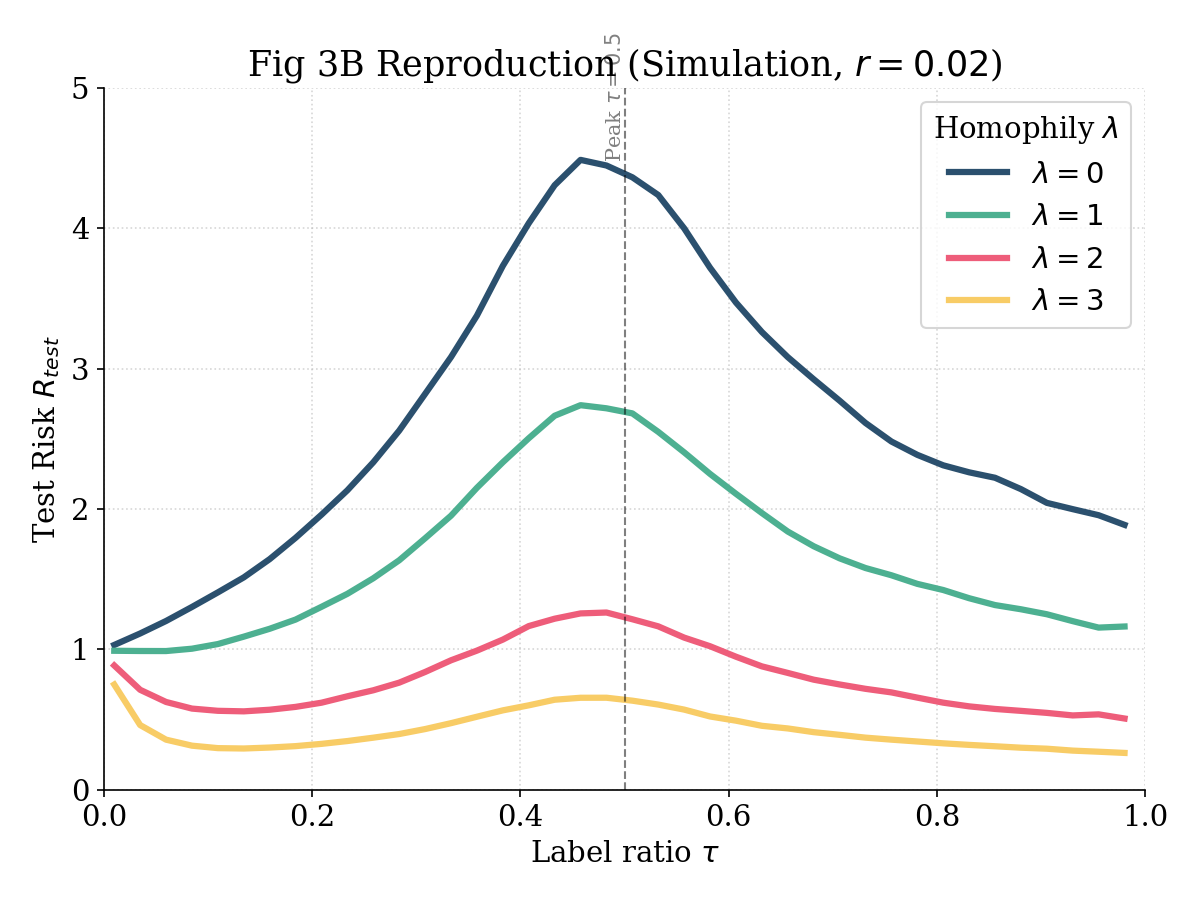
\includegraphics[width=0.7\textwidth]{figure_3b_simulation_5444875.png}
    \caption{Reproduction of homophily-modulated double descent on the CSBM ($r=0.02$). Note the leftward shift of the peak ($\tau \approx 0.4$) away from the theoretical unregularized singularity ($\tau=0.5$).}
    \label{fig:double_descent}
\end{figure}


\section{Extensions}

Having verified the baseline theoretical claims on synthetic data, we now extend our analysis to real-world data.
We probe the limits of the scalar shift and introduce a band-stop spectral operator to isolate signals.

\subsection{Empirical Probe: Asymptotic Sweep on Real-World Graphs}

Traditional machine learning exhibits double descent as the training label ratio $\tau$ varies.
However, as \textcite{shi2024} show, the generalization curve in graph learning is modulated by the extent to which the model attends to the topology.
Therefore, while the original authors focus on $\tau$-sweeps, we swept the scalar shift parameter $c$ to map the limits of their proposed filter.
To evaluate diverse graph structures, we selected two pairs of datasets: Cora and Citeseer (homophilic citation networks) and Chameleon and Squirrel (heterophilic Wikipedia networks).
We ran a linearized GraphSAGE variant (equivalent to Simple Graph Convolution) on them (\texttt{verify\_appendix\_d.py}).
This architecture strips away non-linear activations and degree normalization, reducing the forward pass to a linear operator:
\begin{equation}
    \hat{\mathbf{Y}} = (\mathbf{A} + c\mathbf{I})\mathbf{X}\mathbf{W},
\end{equation}
where $\mathbf{X}$ is the input feature matrix, $\mathbf{W}$ is the weight matrix, and $c$ is the scalar spectral shift. 

The authors theorize that for heterophilic graphs, large values of $|c|$ act as a high-pass filter.
To stress-test this, we swept $c$ from $1$ down to the asymptotic limit $-\infty$.
For the homophilic citation networks, the risk curves successfully reproduced the authors' baseline claims.
Conversely, the heterophilic datasets showed significant deviations.
As $c \to -\infty$, the topological noise degrades the signal, causing the model to abandon the adjacency matrix, converging to a structure-free Multi-Layer Perceptron (MLP) baseline.

\begin{figure}[ht]
    \centering
    % Row 1: Homophilic
    \begin{subfigure}{0.48\textwidth}
        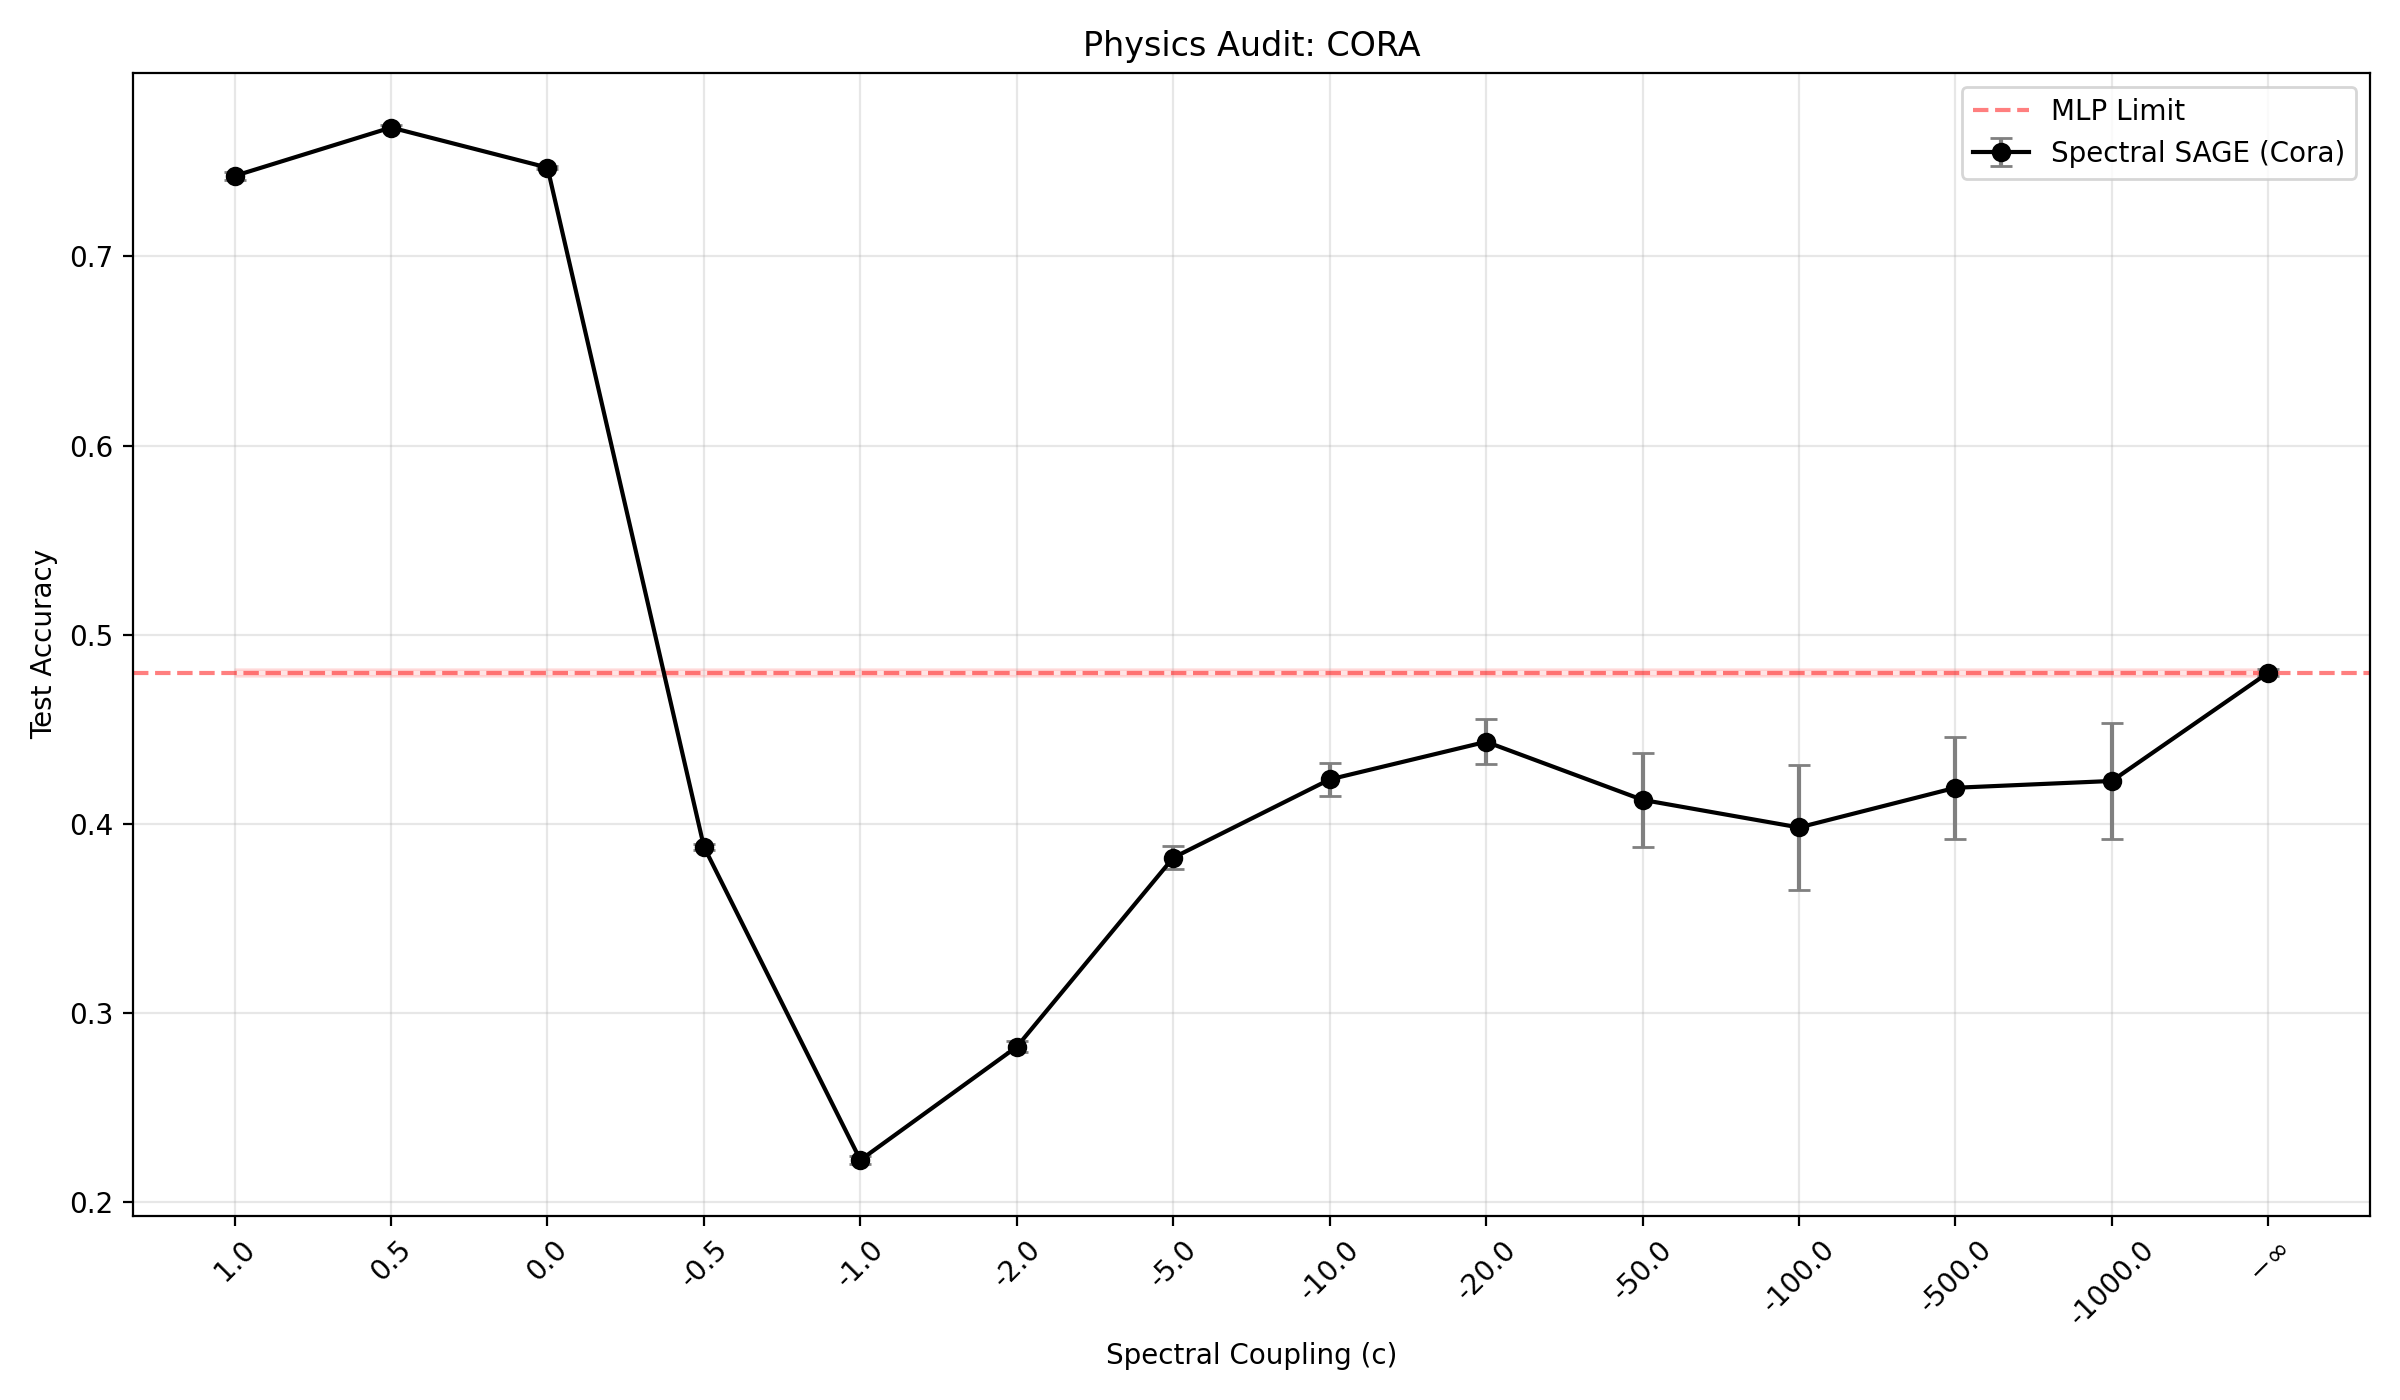
\includegraphics[width=\textwidth]{audit_0_cora.png}
        \caption{Cora (Homophilic)}
    \end{subfigure}
    \hfill
    \begin{subfigure}{0.48\textwidth}
        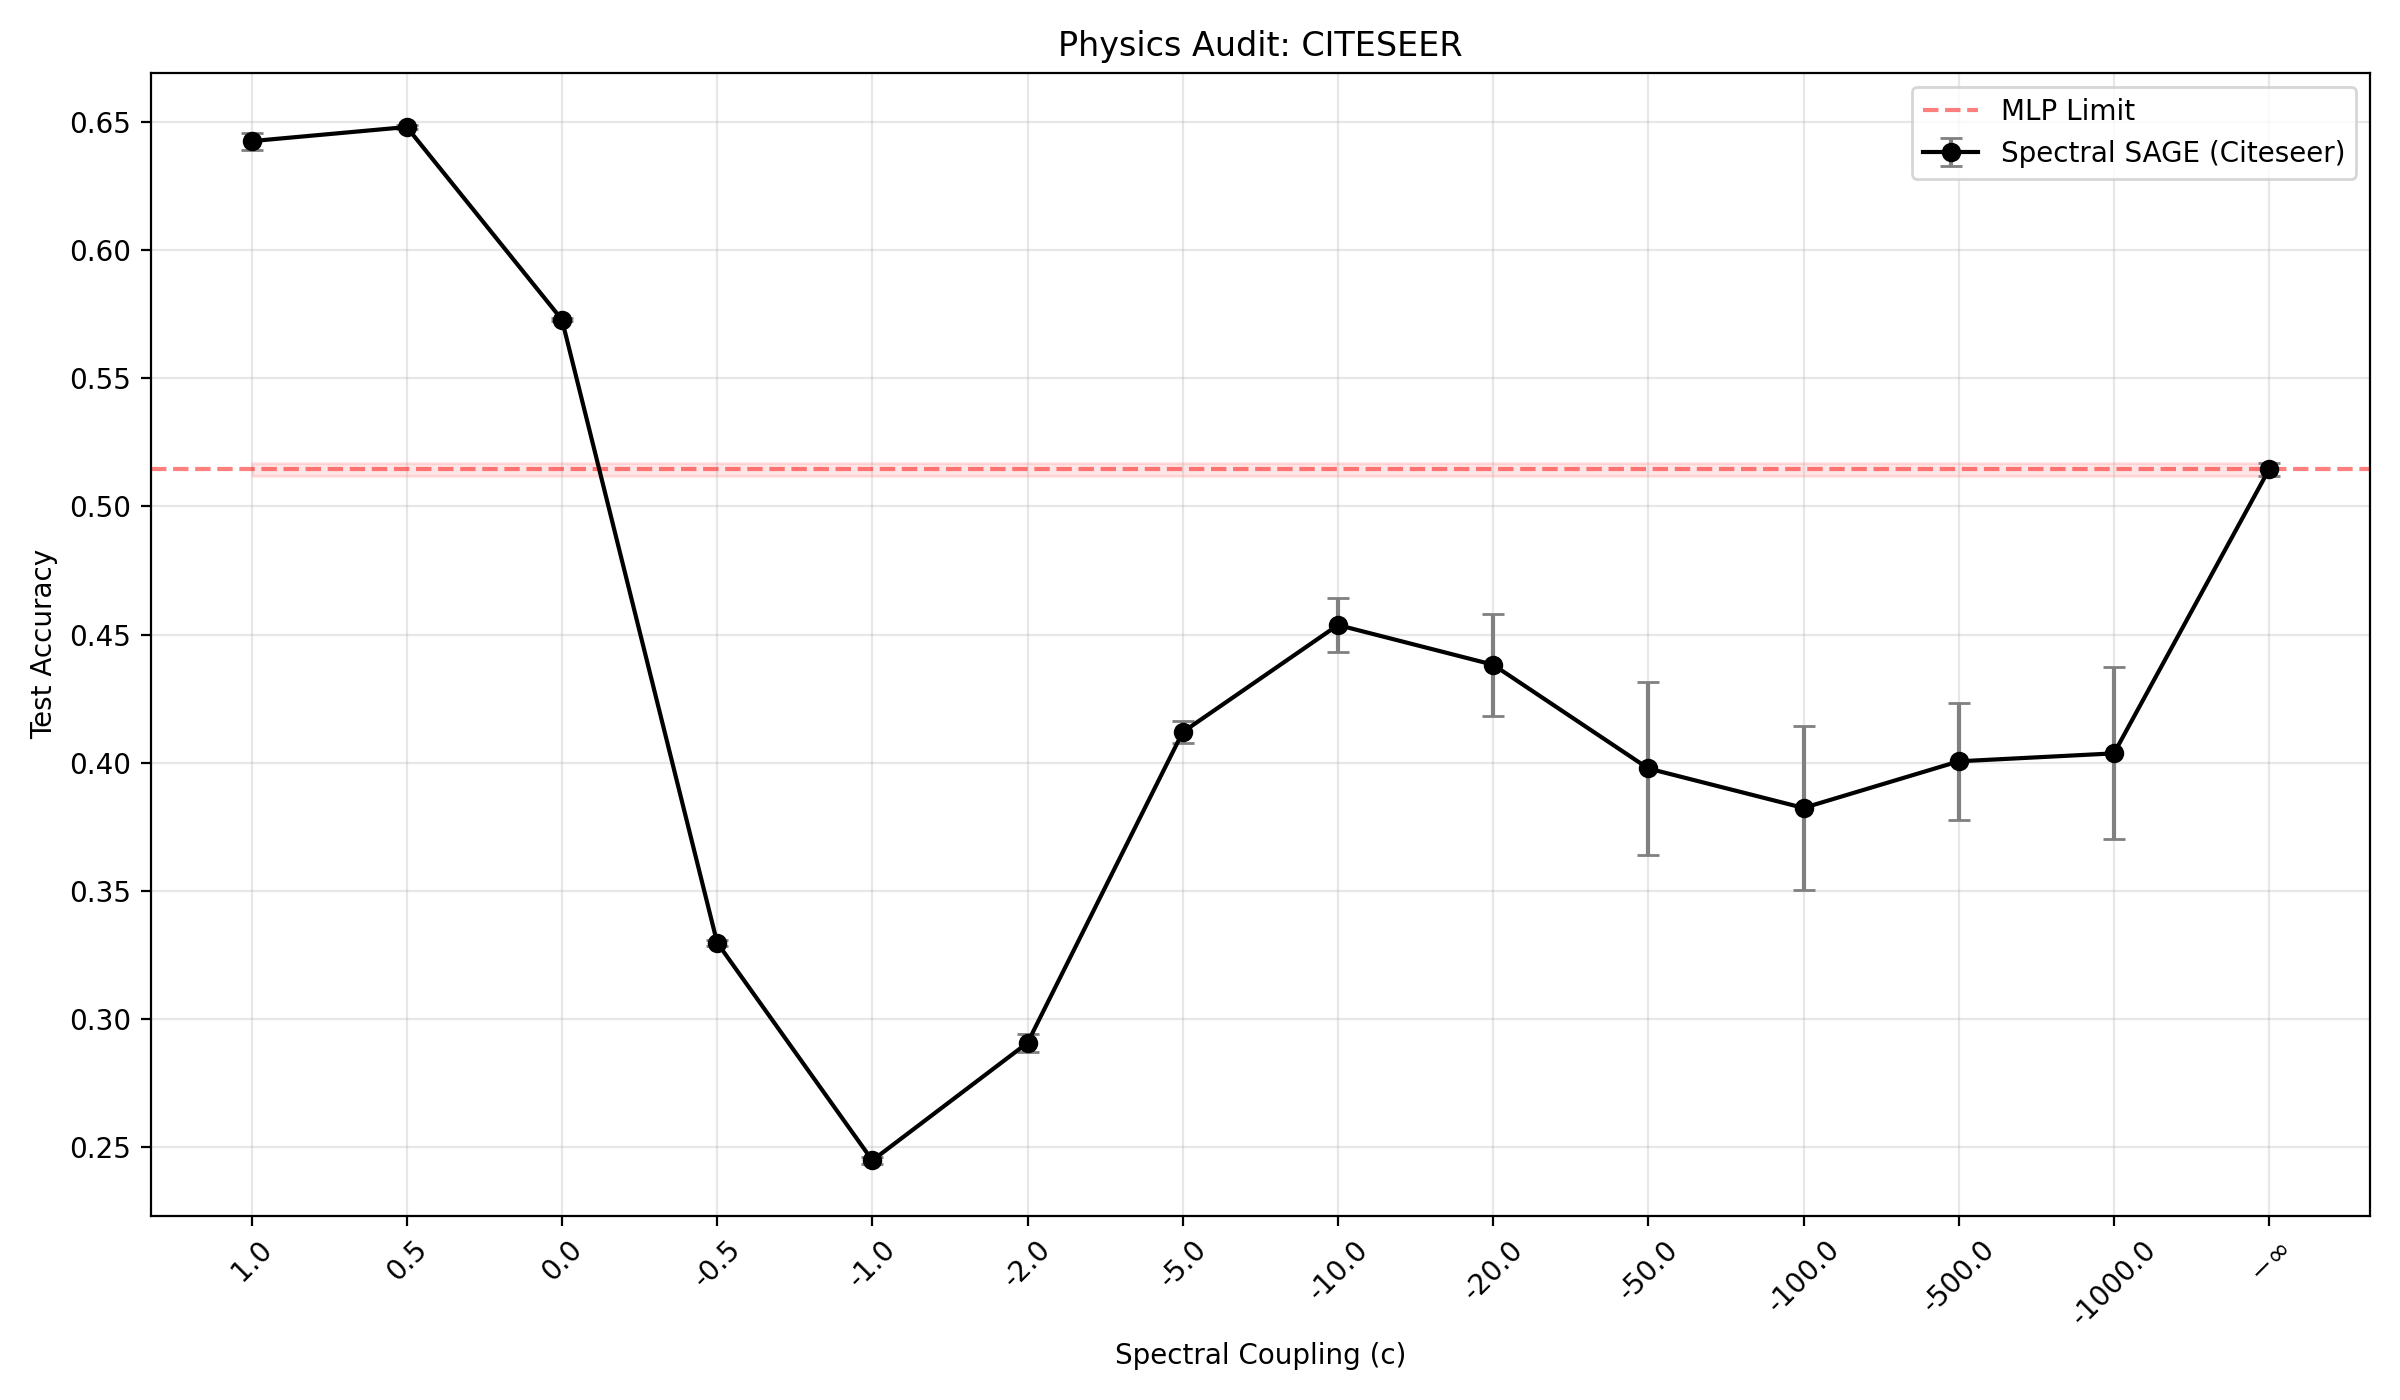
\includegraphics[width=\textwidth]{audit_0_citeseer.png}
        \caption{Citeseer (Homophilic)}
    \end{subfigure}
    
    \vspace{1em} % Adds a little vertical space between rows
    
    % Row 2: Heterophilic
    \begin{subfigure}{0.48\textwidth}
        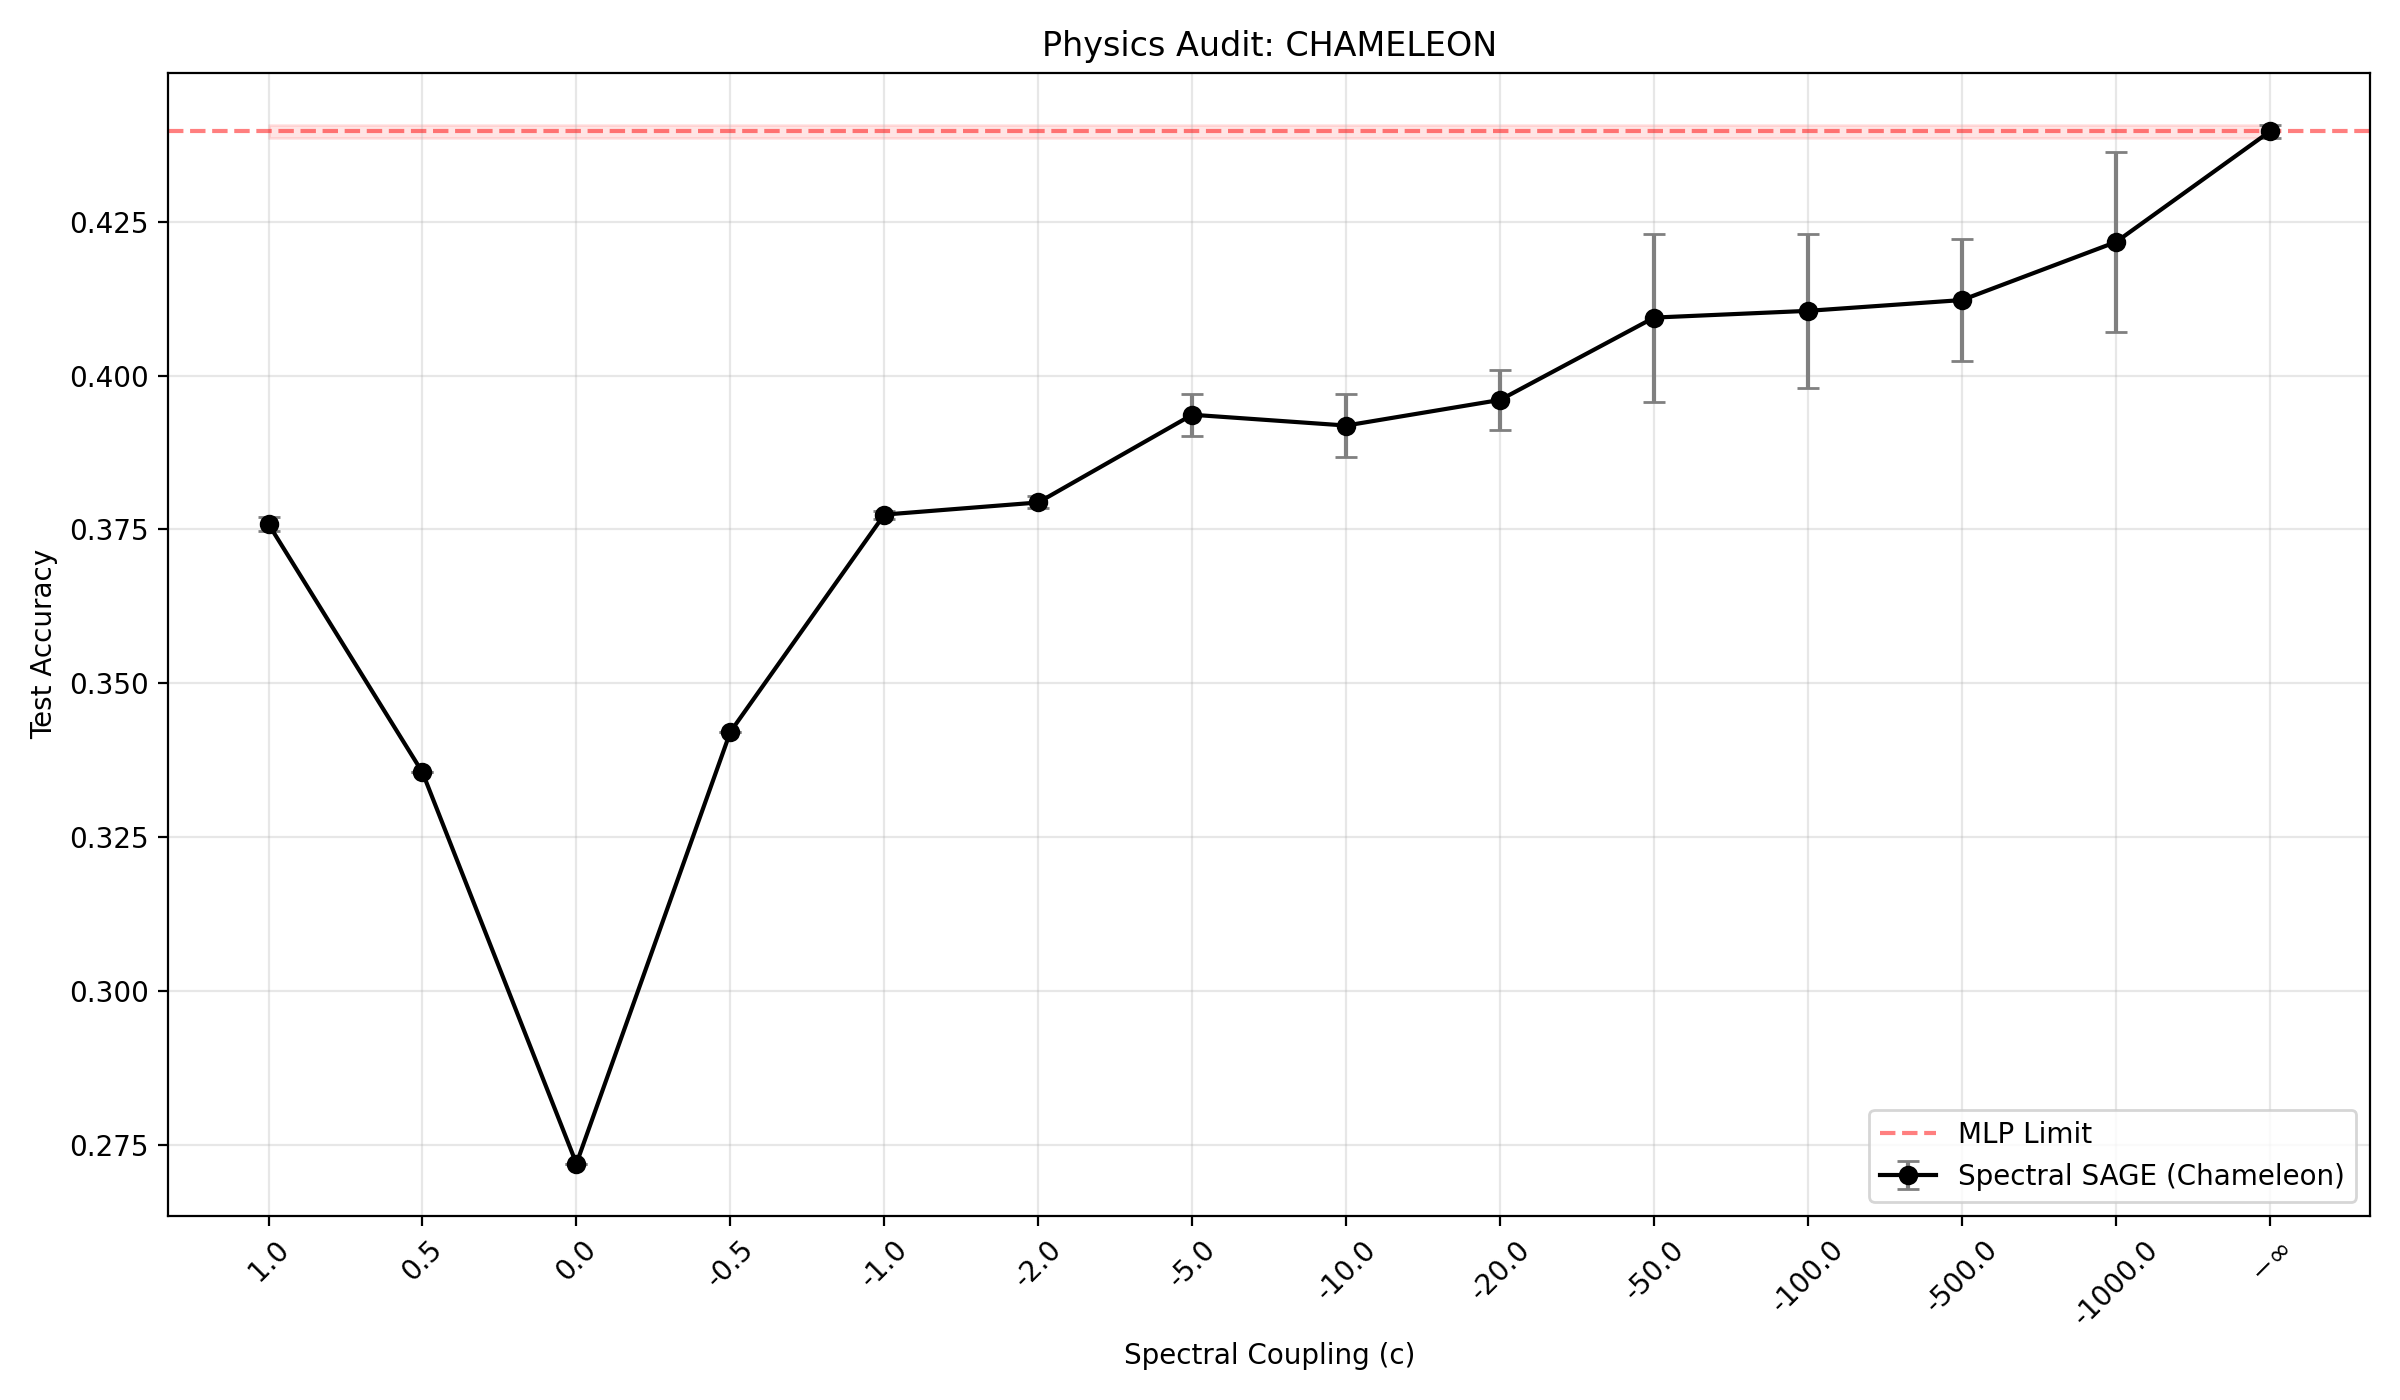
\includegraphics[width=\textwidth]{audit_0_chameleon.png}
        \caption{Chameleon (Heterophilic)}
    \end{subfigure}
    \hfill
    \begin{subfigure}{0.48\textwidth}
        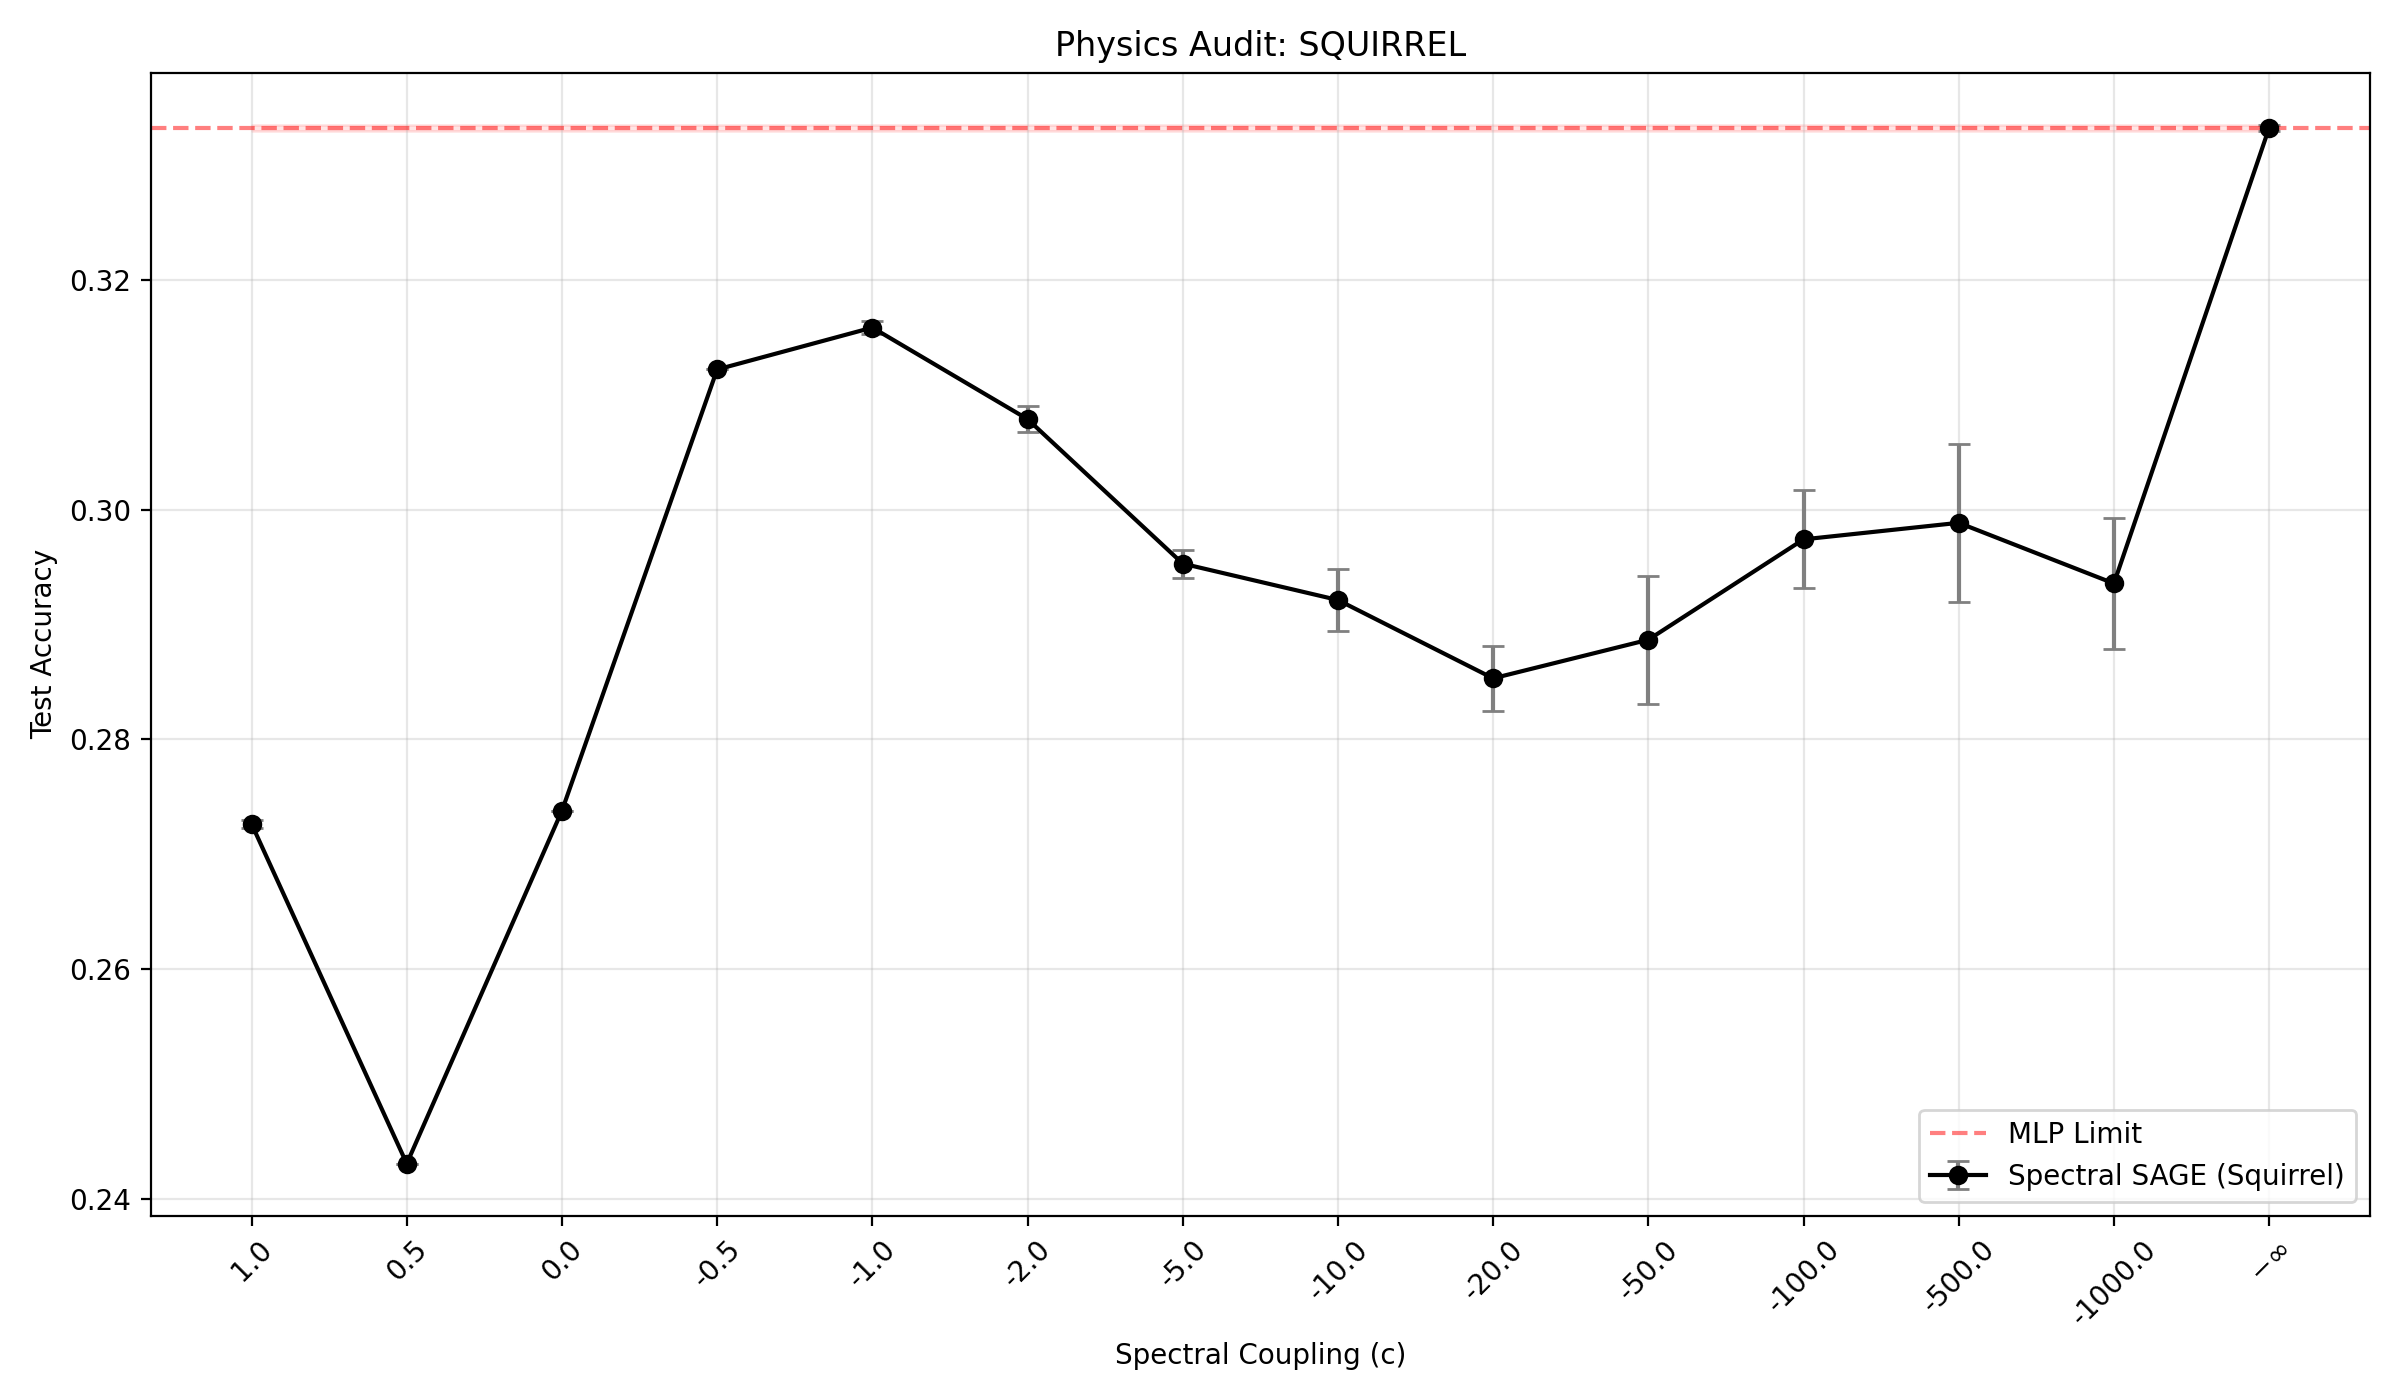
\includegraphics[width=\textwidth]{audit_0_squirrel.png}
        \caption{Squirrel (Heterophilic)}
    \end{subfigure}
    \caption{Test accuracy across the spectral coupling $c$ sweep. In the homophilic graphs (a, b), the optimal filter utilizes the topology. In the heterophilic graphs (c, d), the topological noise acts adversarially, causing the optimal state to diverge to $c \to -\infty$, converging to the structure-free MLP limit (red band).}
    \label{fig:asymptote_sweep}
\end{figure}

\subsection{Empirical Audit: The MLP Boundary Condition}

To test the operational limits of the affine shift, we formalize our analysis through a specific boundary condition test: How does the optimal spectral coupling $c^*$ behave as a real-world graph approaches pure structural noise?

\textcite{shi2024} demonstrate that interpolating a graph's topology toward an Erdős-Rényi random graph accentuates the double descent peak.
We extend this noise-injection framework on the \textit{Texas} dataset using \texttt{audit\_noise.py} to evaluate the stability of the parameter $c$. 

\textbf{Key Finding:} We observe that as noise increases, the optimal spectral coupling diverges to $-\infty$.
Formally, let $\mathbf{H} = (\mathbf{A} + c\mathbf{I})\mathbf{X}\mathbf{W}$ denote the linear network output.
Because the learned weights $\mathbf{W}$ adjust to absorb the magnitude of $c$, we evaluate the normalized limit:
\begin{equation}
    \lim_{c \to -\infty} \frac{1}{c} (\mathbf{A} + c\mathbf{I})\mathbf{X}\mathbf{W} = \lim_{c \to -\infty} \left( \frac{1}{c}\mathbf{A} + \mathbf{I} \right) \mathbf{X}\mathbf{W} = \mathbf{X}\mathbf{W}.
\end{equation}

This algebraic reduction directly challenges the signal processing interpretation provided by \textcite{shi2024} (Appendix D).
They argue that large negative self-loops act as high-pass filters for heterophilic graphs because the spectral distortion ratio between any two signal eigenvalues, $(\lambda_a + c)/(\lambda_b + c)$, approaches $1$ as $c \to -\infty$. 
However, this limit applies to the entire spectrum: for all eigenvalues $\lambda$, the relative response converges to a constant.
By flattening the entire frequency domain, the operator ceases to filter selectively; it converges to a scaled identity matrix ($c\mathbf{I}$). 
Our MLP limit formalized above is the exact spatial consequence of this spectral flattening: the model preserves the signal only by annihilating the graph structure.

As shown in Figure \ref{fig:asymptote_sweep}, this divergence is not limited to synthetic injections.
On the heterophilic Squirrel dataset, the linear probe achieves its global minimum risk at $c \to -\infty$, proving that the linear scalar shift cannot filter the graph; it can only abandon it.

\begin{figure}[ht]
    \centering
    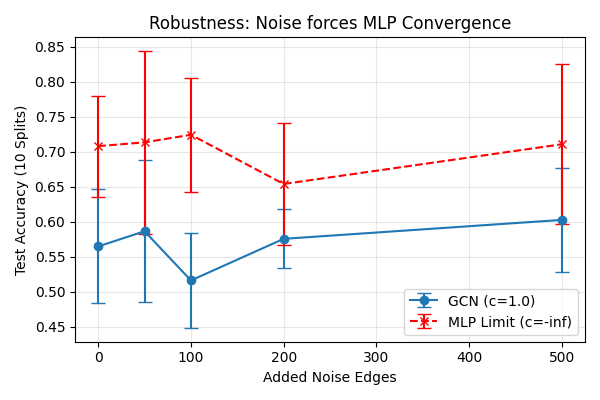
\includegraphics[width=0.6\textwidth]{audit_2_noise_5463380.png}
    \caption{Robustness audit on the Texas dataset. As structural noise edges are injected, the standard GCN ($c=1.0$) degrades and converges toward the theoretical MLP limit ($c \to -\infty$), indicating rejection of the topological signal.}
    \label{fig:noise_audit}
\end{figure}

\subsection{Band-Stop Spectral Filter}

The results of the sweep expose a geometric limitation of $c$.
Mapped to the normalized Laplacian spectrum $\lambda \in [0, 2]$, the affine filter has a frequency response $g(\lambda) = 1 - \lambda + c$.
While our empirical probe utilizes the random-walk matrix $\mathbf{D}^{-1}\mathbf{A}$ for numerical stability, it is similar to the symmetric normalized adjacency $\tilde{\mathbf{A}} = \mathbf{I} - \mathbf{L}$, and they share an identical spectrum.
Because this is a first-order polynomial with a fixed slope, it cannot selectively mask the spectrum.
It lacks the degrees of freedom to mask the noise bulk centered at $\lambda \approx 1$ while preserving the heterophilic signals located at the extremes ($\lambda \approx 0$ and $\lambda \approx 2$).

To resolve this, we propose a \textbf{Band-Stop Filter} $\mathcal{H}$ that selectively performs "surgery" on the spectrum.
In this domain, $\lambda \approx 0$ corresponds to low-frequency homophilic signals, $\lambda \approx 2$ to high-frequency heterophilic signals, and the dense center $\lambda \approx 1$ constitutes a noise bulk \parencite{balcilar2021} (as visualized in Figure \ref{fig:squirrel_spectrum}).
An ideal spectral mask utilizes an indicator function to annihilate the noise bulk centered at $\lambda = 1$ with radius $\epsilon$:
\begin{equation}
    h_{ideal}(\lambda) = \begin{cases} 
      0, & \text{if } |\lambda - 1| \le \epsilon \\
      1, & \text{otherwise} 
   \end{cases}
\end{equation}

Spatial GNN implementations approximate this filter using finite-degree polynomials \parencite{defferrard2016}.
Approximating the step-discontinuity of an indicator function induces the Gibbs phenomenon, causing the polynomial to oscillate and overshoot the $[0, 1]$ bounds \parencite{he2021}.
These frequency ripples leak noise back into the representation. 
To guarantee a stable polynomial approximation, practical implementations relax the hard indicator function into a continuous curve.
The filtered representation space is then computed via matrix projection:
\begin{equation}
\tilde{\mathbf{X}} = \mathbf{U} h(\mathbf{\Lambda}) \mathbf{U}^\top \mathbf{X}.
\end{equation}

By damping the eigenvalues in the $(1-\epsilon, 1+\epsilon)$ range, this isolates the signal.
Evaluating this requires a full eigendecomposition of the Laplacian, which scales computationally at $\mathcal{O}(n^3)$ \parencite{kipf2017}.

\begin{figure}[ht]
    \centering
    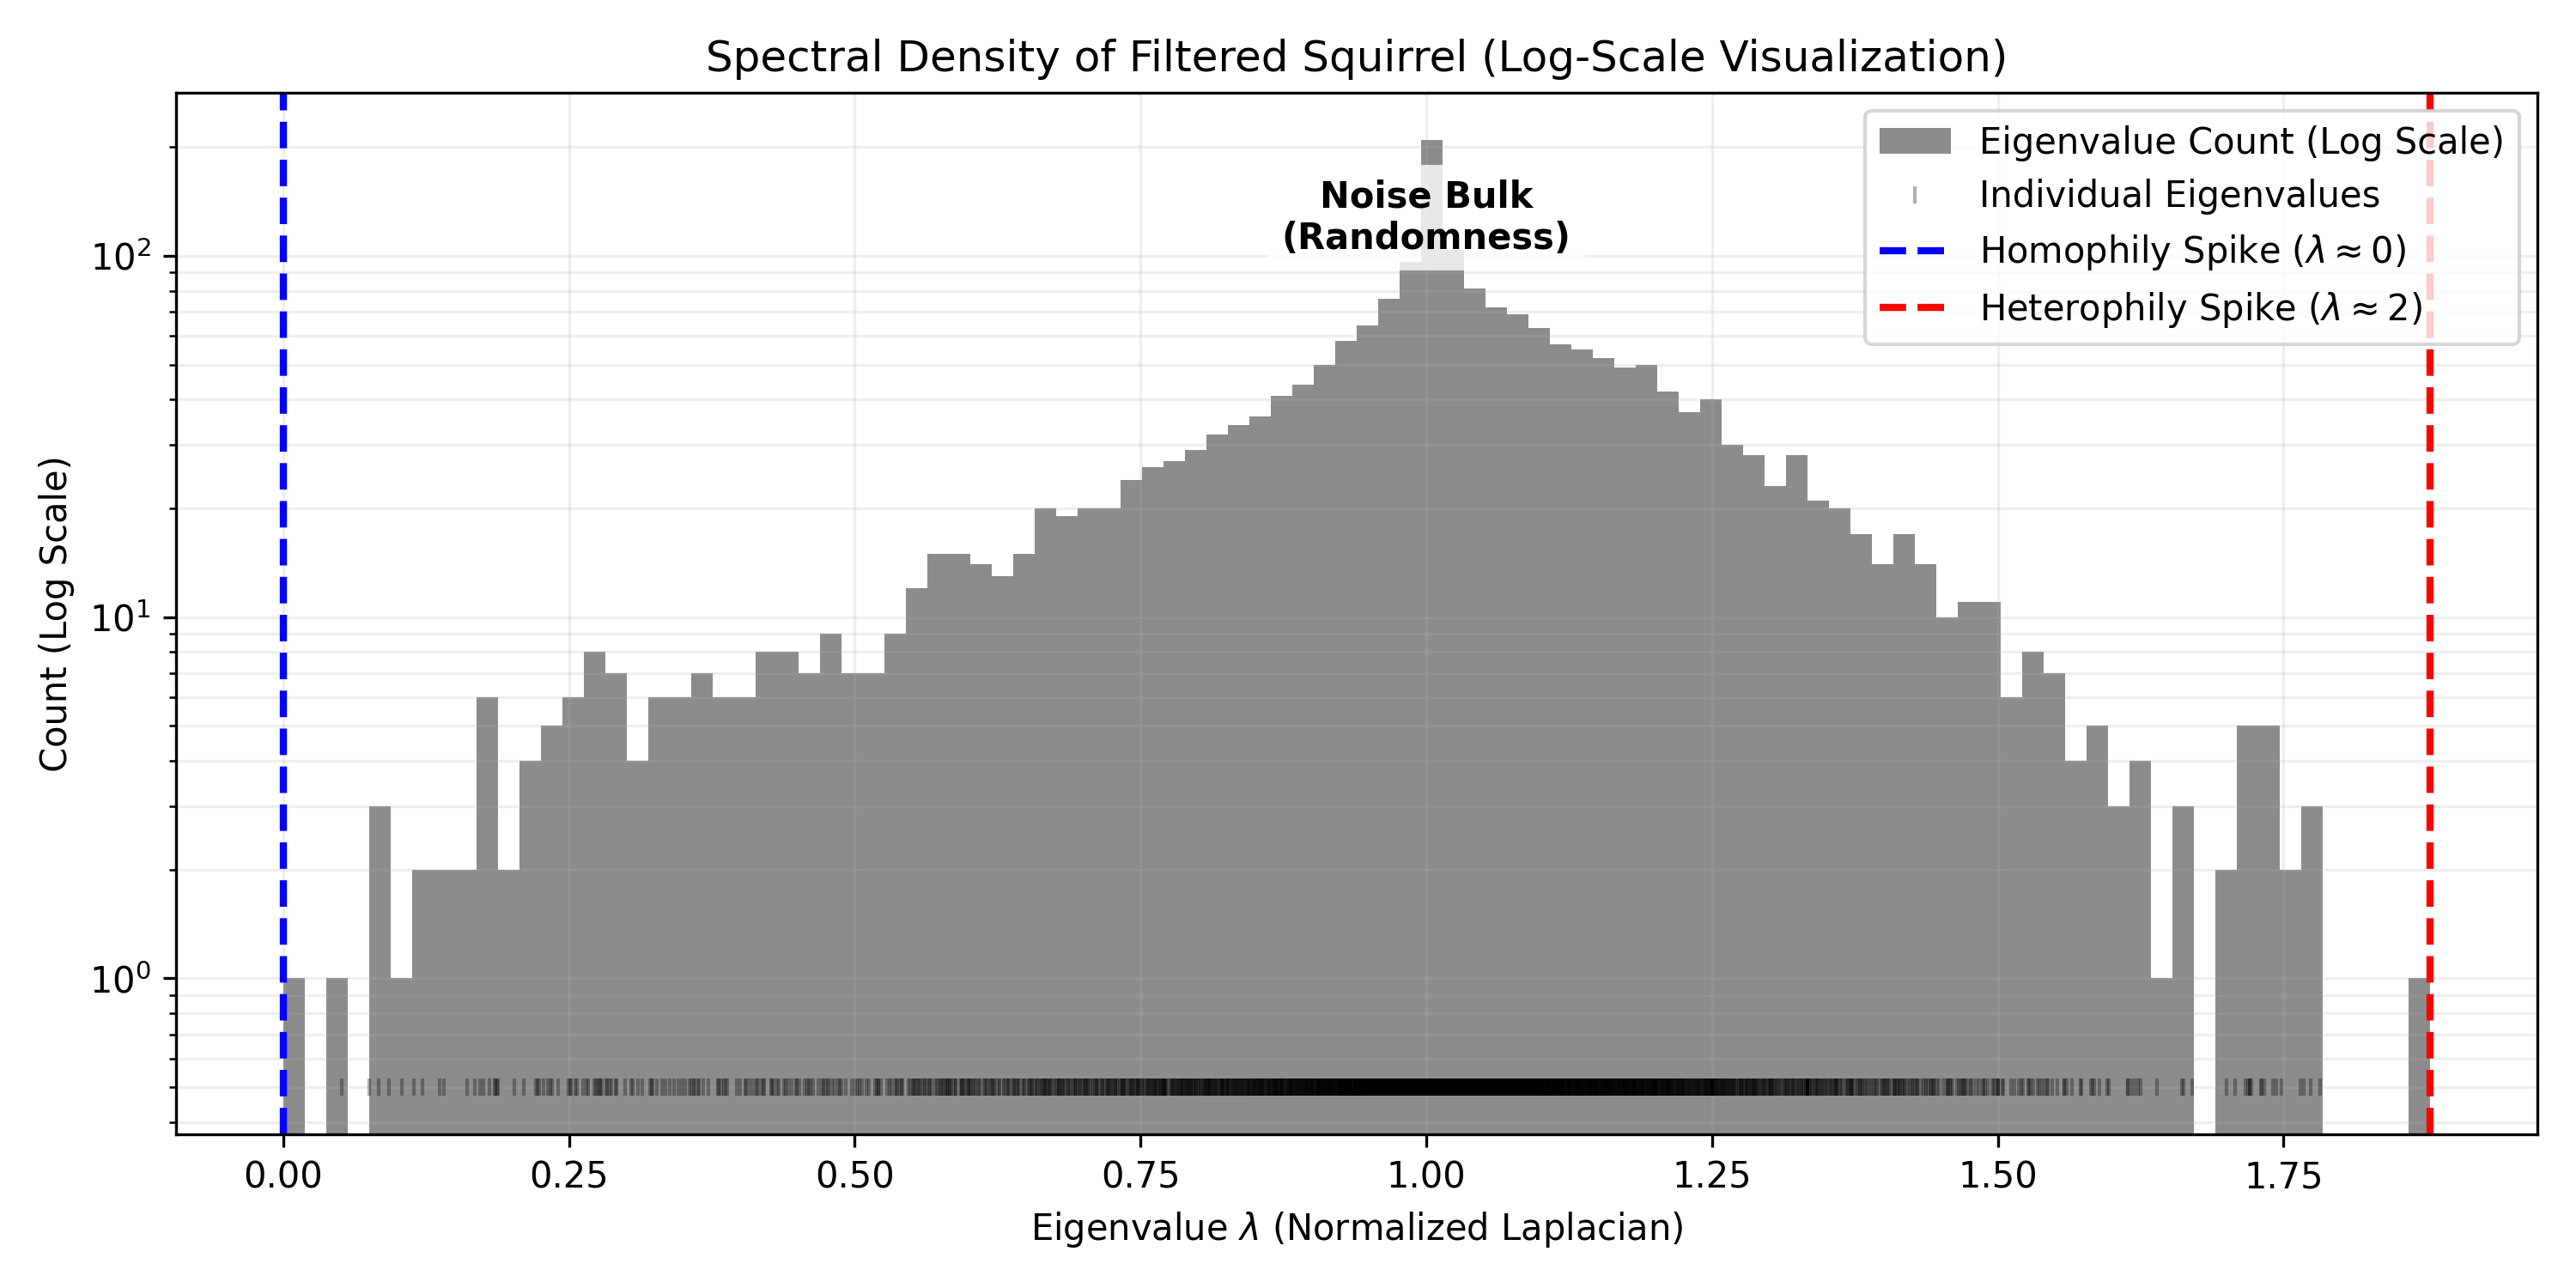
\includegraphics[width=0.7\textwidth]{squirrel_spectrum_log.png}
    \caption{Spectral density of the normalized Laplacian for the Platonov-filtered Squirrel dataset (log scale). The structural distribution is overwhelmingly concentrated in the uninformative topological noise bulk ($\lambda \approx 1$). The band-stop filter annihilates this central region, preserving only the latent community eigenspaces near the domain boundaries ($\lambda \approx 0$ and $\lambda \approx 2$).}
    \label{fig:squirrel_spectrum}
\end{figure}

\subsection{Results on Heterophilic Benchmark}

We evaluated a band-stop filter on the \textit{Squirrel} dataset.
Crucially, while \textcite{shi2024} evaluate their scalar filter on the original benchmark datasets (the original Squirrel containing 5201 nodes, reporting artificially inflated accuracies $>70\%$), we use the deduplicated variant introduced by \textcite{platonov2023} (the filtered Squirrel containing 2223 nodes).
The original heterophilic datasets leak train-test data via duplicate node features.
By utilizing the filtered Platonov splits, we eliminate this leakage.
Consequently, the baseline accuracies are substantially lower, but represent realistic measures of heterophilic generalization.
Furthermore, to ensure the algebraic definition $P(\mathbf{A}) = \mathbf{A} + c\mathbf{I}$ strictly maps to the evaluation, we strip all pre-existing self-loops from the graph prior to filtering (\texttt{remove\_self\_loops}).
Without this sanitization, native self-loops silently compound with the tunable parameter $c$, invalidating the controlled frequency response.

\begin{itemize}[leftmargin=*]
    \item \textbf{Structure-Free MLP:} 33.4\% Accuracy.
    \item \textbf{Standard GCN:} 32.7\% Accuracy.
    \item \textbf{Shi et al. (Optimized $c$):} 34.1\% Accuracy.
    \item \textbf{Band-Stop filter:} \textbf{38.3\%} Accuracy.
\end{itemize}

These accuracies are notably lower than those reported in earlier heterophily literature ($>70\%$), reflecting the lack of data leakage in the Platonov-filtered splits. 
On these benchmarks, even state-of-the-art architectures (e.g., GPRGNN \parencite{chien2021} or H2GCN \parencite{zhu2020}) typically achieve results in the $35\%$-$45\%$ range. 
The fact that our linear Band-Stop Filter achieves $38.3\%$ demonstrates that much of the performance gain in specialized heterophilic GNNs can be attributed to the selective suppression of the central noise bulk, rather than complex non-linear feature interactions.

This result contextualizes the practical limits of the affine shift.
While Shi et al.'s non-linear implementation slightly outperforms the structure-free baseline (34.1\% vs 33.4\%), the band-stop filter can find something (38.3\%) in valid heterophilic regimes.


\section{Conclusion}
We have demonstrated that, while the scalar filter $\mathbf{A} + c\mathbf{I}$ explains double descent in homophilic regimes, it is geometrically insufficient for signal recovery in true heterophilic networks.
Faced with dense noise, optimization forces the linear model to disconnect the graph entirely ($c \to -\infty$).

To resolve this, we proposed a Band-Stop Spectral Filter, which trims noisy eigenspaces.
Our implementation used the full eigendecomposition (\texttt{torch.linalg.eigh}), which has $\mathcal{O}(n^3)$ complexity.
Future work may focus on scaling this operator to larger graphs using polynomial approximations of order $K$ (e.g., ChebNet \parencite{defferrard2016}).
However, designing a polynomial with a sufficiently sharp "cut" to suppress the noise bulk requires a high degree $K$.
If $K$ exceeds the graph's diameter, the filter loses its spatial locality and collapses into a global operator, ignoring the relational structure of the graph \parencite{levie2018}.

\printbibliography

\section*{Appendix: Algorithms and Experiment Protocols}

To differentiate graph effects from stochastic optimization, we implemented all experiments in PyTorch Geometric and NumPy. Table \ref{tab:architecture} summarizes the architectural differences between our linear probe and the benchmark methodologies.

\begin{table}[h]
\centering
\caption{Architectural comparison distinguishing standard performance benchmarks, Shi et al.'s theoretical replica limits, and our linear probe.}
\label{tab:architecture}
\renewcommand{\arraystretch}{1.5}
\setlength{\tabcolsep}{10pt}
\begin{adjustbox}{max width=\textwidth}
\begin{tabular}{l l l l}
\toprule
\textbf{Feature} & \textbf{\begin{tabular}[t]{@{}l@{}}1. Standard GCN\\(Benchmark)\end{tabular}} & \textbf{\begin{tabular}[t]{@{}l@{}}2. Shi et al. \\(Analytical Theory)\end{tabular}} & \textbf{\begin{tabular}[t]{@{}l@{}}3. Spectral SAGE\\(Our Probe)\end{tabular}} \\
\midrule
\textbf{Equation} & $\mathbf{Z} = \underbrace{\tilde{\mathbf{A}}}_{\text{Filter}} \sigma(\underbrace{\tilde{\mathbf{A}}}_{\text{Filter}} \mathbf{X}\mathbf{W}_1) \mathbf{W}_2$ & $\mathbf{Z} = \underbrace{(\mathbf{D}^{-1/2}\mathbf{A}\mathbf{D}^{-1/2} + c\mathbf{I})}_{\text{Tunable Filter}} \mathbf{X}\mathbf{W}$ & $\mathbf{Z} = \underbrace{(\mathbf{D}^{-1}\mathbf{A} + c\mathbf{I})}_{\text{Tunable Filter}} \mathbf{X}\mathbf{W}$ \\
\rowcolor{gray!10} \textbf{Depth} & \textbf{2-Layer} (Multi-Hop) & \textbf{1-Layer} (Single-Hop) & \textbf{1-Layer} (Single-Hop) \\
\textbf{Non-Linearity} & \textbf{ReLU} (Mixes Frequencies) & \textbf{None} (Linear) & \textbf{None} (Linear) \\
\rowcolor{gray!10} \textbf{Normalization} & Symmetric ($\tilde{\mathbf{D}}^{-1/2}\tilde{\mathbf{A}}\tilde{\mathbf{D}}^{-1/2}$) & Symmetric ($\mathbf{D}^{-1/2}\mathbf{A}\mathbf{D}^{-1/2}$) & \textbf{Random Walk} ($\mathbf{D}^{-1}\mathbf{A}$) \\
\textbf{Role} & \textbf{Performance} (SOTA) & \textbf{Analysis} (Theory) & \textbf{Audit} (Signal Isolation) \\
\bottomrule
\end{tabular}
\end{adjustbox}
\end{table}

\textbf{1. CSBM Data Generation and Ridge Regression:} To reproduce the analytical double descent curves (Figure \ref{fig:double_descent}), we implemented the CSBM simulation as defined by the replica limits.
Algorithm \ref{alg:csbm} details the generation of spiked covariance features and the symmetric Gaussian adjacency matrix, evaluated via closed-form regularized normal equations.

\textbf{2. The Spectral SAGE Probe:} To sweep $c \to -\infty$ (Figure \ref{fig:asymptote_sweep}), we implemented a custom \texttt{MessagePassing} probe (Algorithm \ref{alg:spectral_probe}) based on GraphSAGE that applies random-walk normalization ($\mathbf{D}^{-1}\mathbf{A}$) via \texttt{aggr='mean'} before adding the scalar shift.

\textbf{3. Topological Noise Injection:} To evaluate the boundary conditions of the affine shift (Figure \ref{fig:noise_audit}), we developed an iterative structural noise injector (Algorithm \ref{alg:noise_injection}).
This protocol gradually degenerates the \textit{Texas} dataset with random edges and observes how the optimizer shifts the parameter $c^*$ as the graph SNR collapses.

\textbf{4. Empirical Baseline Reproductions:} To establish a foundation before extending the theoretical limits, we reproduced the double descent curves for the Cora network (Figure 1 in Shi et al.) and the structural noise injections on the Chameleon dataset (Figure 2d). These implementations (\texttt{reproduce\_fig\_1\_cora.py}, \texttt{reproduce\_fig\_2d.py}) replicate the original paper's non-standard evaluation protocols, including the use of Mean Squared Error on one-hot encoded targets, unnormalized feature matrices, and custom stratified sampling to prevent class collapse.

The complete, reproducible implementation suite is available at: \url{https://github.com/zetrozky/spectral-limits-on-graphs}

\begin{algorithm}[H]
\caption{CSBM Generation \& Ridge Evaluation (\texttt{reproduce\_fig\_3b.py})}
\label{alg:csbm}
\KwIn{Nodes $N$, Features $d$, Feature SNR $\mu$, Spectral Separation $\lambda$, Ridge $r$}
\KwOut{Empirical Test Risk}
\BlankLine
\tcp{1. Ground Truth and Spiked Covariance Features}
$\mathbf{y} \leftarrow \text{Half } +1, \text{Half } -1$\;
$\mathbf{u} \leftarrow \text{Gaussian}(0, \mathbf{I}_d) / \|\mathbf{u}\|_2$\;
$\mathbf{Z}_x \leftarrow \text{Gaussian}(0, \mathbf{I}) / \sqrt{d}$\;
$\mathbf{X} \leftarrow \sqrt{\mu / N} (\mathbf{y} \mathbf{u}^\top) + \mathbf{Z}_x$\;

\BlankLine
\tcp{2. Symmetric Gaussian Graph Topology}
$\mathbf{Z}_A \leftarrow \text{Gaussian}(0, \mathbf{I}_{N \times N})$\;
$\mathbf{A} \leftarrow (\mathbf{Z}_A + \mathbf{Z}_A^\top) / \sqrt{2N}$\;
$\mathbf{A} \leftarrow \mathbf{A} + (\lambda / N)(\mathbf{y} \mathbf{y}^\top)$\;

\BlankLine
\tcp{3. Filter and Solve Normal Equations}
$\tilde{\mathbf{X}} \leftarrow \mathbf{A}\mathbf{X}$ \tcp*{Evaluate pure topological filter}
$\mathbf{w}^* \leftarrow (\tilde{\mathbf{X}}_{train}^\top \tilde{\mathbf{X}}_{train} + r\tau\mathbf{I})^{-1} \tilde{\mathbf{X}}_{train}^\top \mathbf{y}_{train}$\;
\Return{$\text{MSE}(\tilde{\mathbf{X}}_{test}\mathbf{w}^*, \mathbf{y}_{test})$}\;
\end{algorithm}

\vspace{1em}

\begin{algorithm}[H]
\caption{Linear Spectral Probe
(\texttt{verify\_appendix\_d.py})}
\label{alg:spectral_probe}
\KwIn{Edge Index $\mathcal{E}$, Node Features $\mathbf{X}$, Labels $\mathbf{y}$, Shift $c$}
\KwOut{Test Accuracy at minimum training loss}
\BlankLine
$\mathcal{E}_{pruned} \leftarrow \text{remove\_self\_loops}(\mathcal{E})$\;
\SetKwFunction{FForward}{forward}
\SetKwProg{Fn}{Function}{:}{}
\Fn{\FForward{$\mathbf{X}$, $\mathcal{E}_{pruned}$, $c$}}{
    $\mathbf{H}_{agg} \leftarrow \text{propagate}(\mathcal{E}_{pruned}, \mathbf{X}, \text{aggr='mean'})$ \tcp*{$\mathbf{D}^{-1}\mathbf{A}\mathbf{X}$}
    $\mathbf{Z} \leftarrow \mathbf{H}_{agg} + c\mathbf{X}$ \tcp*{Apply scalar shift}
    \Return{$\mathbf{Z}\mathbf{W}$} \tcp*{Single linear projection}
}
\tcp{Optimize via Adam and CrossEntropyLoss over 200 epochs...}
\end{algorithm}

\vspace{1em}

\begin{algorithm}[H]
\caption{Structural Noise Injection Protocol (\texttt{audit\_noise.py})}
\label{alg:noise_injection}
\KwIn{Clean Graph $\mathcal{G}(\mathcal{V}, \mathcal{E})$, Noise Steps $\mathcal{S}$}
\KwOut{Accuracy trajectory for standard ($c=1$) and MLP limit ($c=-\infty$)}
\BlankLine
$\mathcal{E}_{base} \leftarrow \text{remove\_self\_loops}(\mathcal{E})$\;
\For{$n_{edges} \in \mathcal{S}$}{
    $\mathcal{E}_{noise} \leftarrow \text{Sample Uniform}(|\mathcal{V}| \times |\mathcal{V}|, \text{size}=n_{edges})$\;
    $\mathcal{E}_{corrupted} \leftarrow \mathcal{E}_{base} \cup \mathcal{E}_{noise}$\;
    
    $\text{Acc}_{GCN} \leftarrow \text{Evaluate(Algorithm \ref{alg:spectral_probe} with } \mathcal{E}_{corrupted}, c=1.0)$\;
    $\text{Acc}_{MLP} \leftarrow \text{Evaluate(Algorithm \ref{alg:spectral_probe} with } \mathcal{E}_{corrupted}, c=-1000.0)$\;
    
    $\text{Log}(\text{Acc}_{GCN}, \text{Acc}_{MLP})$\;
}
\end{algorithm}

\end{document}